Until this point, this section mainly focused on establishing statistical preconditions before it is possible to acquire cross-correlation. If the previous steps would be left out, the correlation would be much more likely to report erroneous results, e.g. spurious correlation. For calculating a bivariate correlation, Pearson's $r$ \eqref{formula:pearson_r}, will be used in the following.

% https://drive.google.com/file/d/1EKf_rly5OQ-oTts61HDeddYCwuBZLd1n/view

In order to make the danger of spurious correlation more tangible, Figure~\ref{fig:spurious_regression} shows an example for two stock prices which are not preprocessed. While the correlation on the plain stock prices appears very high with $r=0.96$, it is rather not existing at all after the preprocessing steps of differencing, transformation, normalization and modelling. This indicates that the first observed $r$ is high due to the autocorrelation of the both time series and their shared exogenous variable, i.e. the overall market performance.

\begin{figure}[!ht]
    \centering
    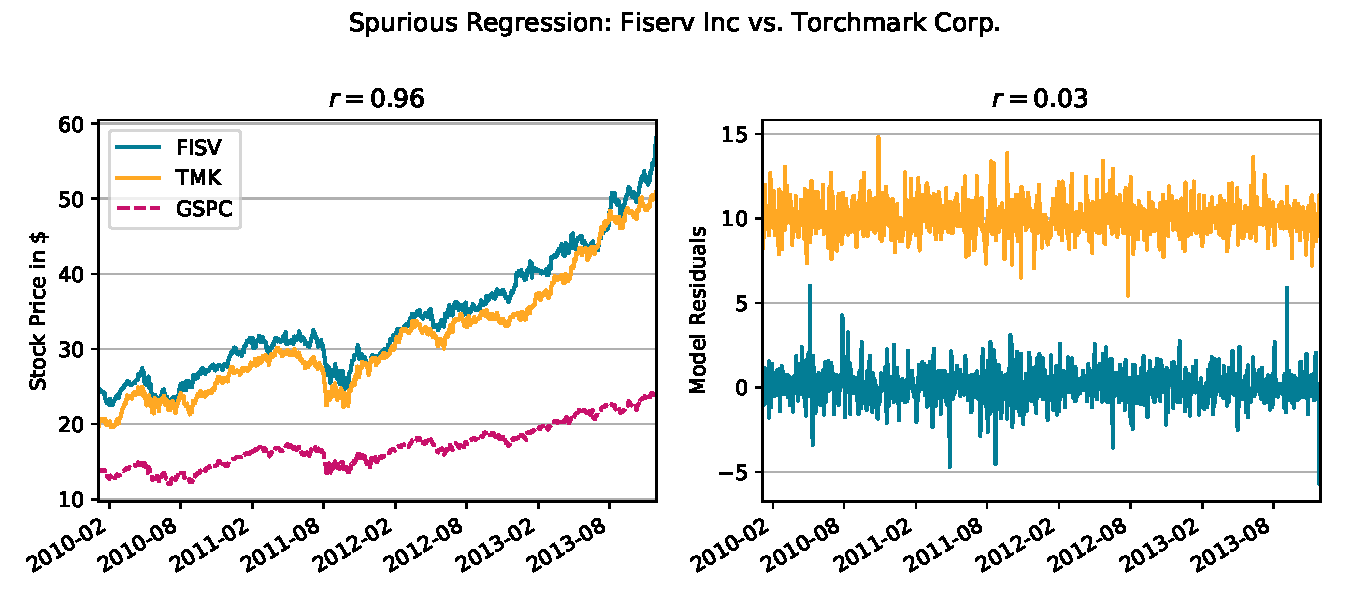
\includegraphics[width=\textwidth]{figures/regression/spurious-FISV-TMK.pdf}
    \caption{Data for the two companies \emph{Fiserv} and \emph{Torchmark}. The left plot shows the unmodified daily opening prices which revealed a Cross-Correlation of $r=0.99$. Additionally a scaled and shifted version of the market index is plotted. The right plot shows the same time series after properties like autocorrelation and heteroscedasticity were removed which led to $r=0.06$. For the sake of visibility, the orange time series is increased by 10.}
    \label{fig:spurious_regression}
\end{figure}

Even though $r$ is a very popular measure, it needs to be borne in mind that this measure does not account for nonlinear relationship which is not always a sufficient assumption. Therefore, the observed value might not fully reflect the real correlation but rather can be interpreted as an approximation. Since this limitation holds for all correlation values in this experiment, the values can fairly be compared to each other.

To see the impact of the several preprocessing steps, $r$ is calculated for each pair of stocks from four different phases. The distribution of $r$ for the original daily open prices, intraday returns, normalized returns and the residuals of the autoregressive models is visualized by violin plots in Figure~\ref{fig:steps-correlations-ind}. Because 467 stock prices are considered, there are 108.811 different pairs of stocks in total. With this high number of samples, the critical values for the 95~\% confidence interval are -0.006 and 0.006 respectively. Even for a more restrictive interval with $\alpha = 0.0001$, i.e. 99.99~\% confidence, the critical values are only -0.012 and 0.012 which for the whitened data in the last step still leads to 86~\% of all samples being significant. In consideration of this ever-present significance of correlation coefficients, the values are not evaluated by such confidence levels.

% Using the Student's $t$ distribution for the correlation coefficients

Except for autoregressive modelling, the distribution changes drastically with each preprocessing step. Initially, $r$ revealed a median of 0.48 and a great number of extreme values for the original stock prices. As the second distribution for price returns shows, this step does not tackle spurious correlation in a great manner. No pair of stocks is negatively correlated with each other since all stocks include the performance of the overall market or even the industry segment. After the exogenous impact was filtered out to a great extent, a more realistic distribution with a zero median can be observed. In general, stock prices share no more correlation with each other than the market performance and therefore reveal a coefficient close to zero. Relatively few stocks show a greater relationship which can be of a positive nature as well as of a negative nature.

\begin{figure}[!ht]
    \centering
    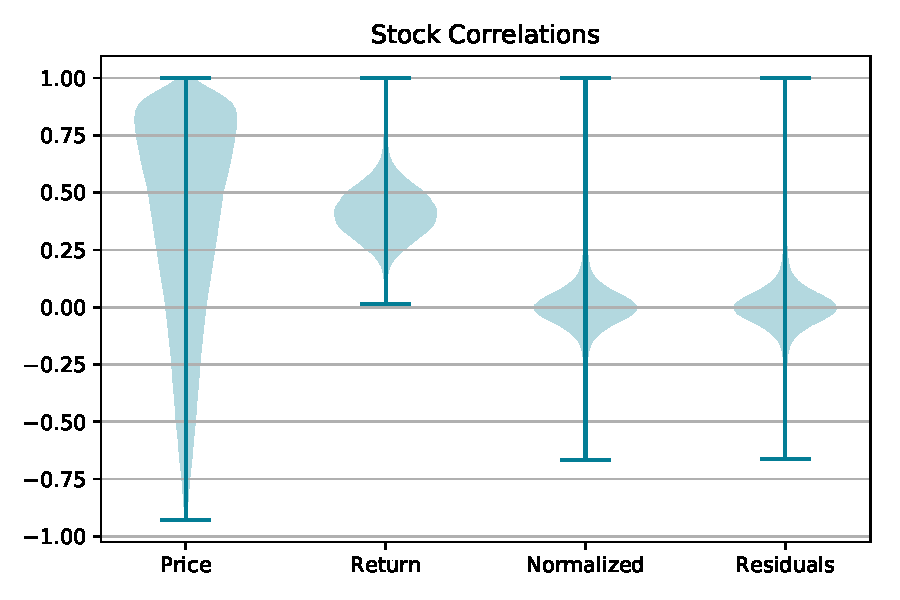
\includegraphics[width=0.8\textwidth]{figures/regression/steps-correlations-ind-norm.pdf}
    \caption{Violin plot of cross-correlation distributions for four main preprocessing steps. The filled area visualizes the approximated data distribution along the vertical line.}
    \label{fig:steps-correlations-ind}
\end{figure}

As mentioned in Section~\ref{subsubsection:processing:exogenous} the price returns can also be normalized by the S\&P~500 market index instead of separate industry means. For this alternative normalization method, the violin plots are shown in Figure~\ref{fig:steps-correlations-gspc}. Compared to the primary normalization by industry, the distribution is not located around zero but reveals a median of 0.2. Because all stocks are positively correlated with each other, this leads to the conclusion that not all exogenous influences are removed and therefore lead to spurious correlation. Concluding, the industry-wise normalization is preferable over market-wise normalization if one is interested in the cross-correlations among stocks from the same stock exchange.

\begin{figure}[!ht]
    \centering
    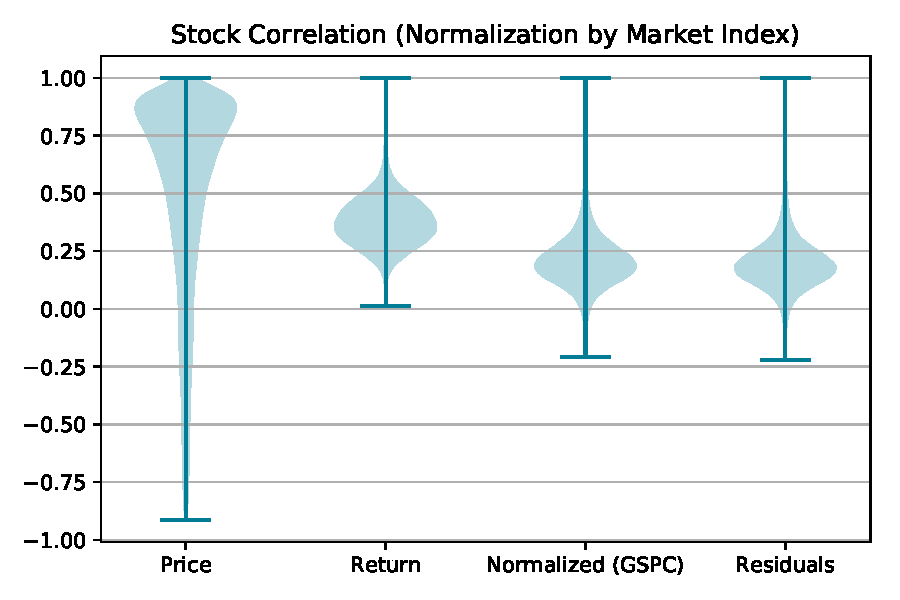
\includegraphics[width=0.8\textwidth]{figures/regression/steps-correlations-gspc-norm.pdf}
    \caption{Violin plot of cross-correlation distributions for four main preprocessing step with the normalization being adapted for market-wise instead of industry-wise normalization.}
    \label{fig:steps-correlations-gspc}
\end{figure}


\paragraph{Correlation Graph}

In order to visualize and inspect the calculated cross-correlations, a graph is defined and visualized in Figure~\ref{fig:graph-correlations}. As stated earlier in this section, there is a tremendous number of significant correlations. If all these correlations would be considered, the plotted graph would become unmanageable. Instead, the 99.9th percentile of all absolute correlation coefficients is calculated which equals 0.3688. Only positive or negative values outside of this percentile are considered for visualization. This leads to 109 correlations among 123 different stocks from all industry sectors. A node's size is determined respectively to its total revenue in 2010 in order to indicate its importance.

On this rather small and incomplete graph, individual nodes, connections and communities in the form of subgraphs can be further examined. It should be noted that the graph consists of the most extreme values and therefore is not a representative sample for the entire graph which would reveal an unmanageable number of edges.

\begin{figure}
    \centering
    \begin{subfigure}{\textwidth}
        \centering
        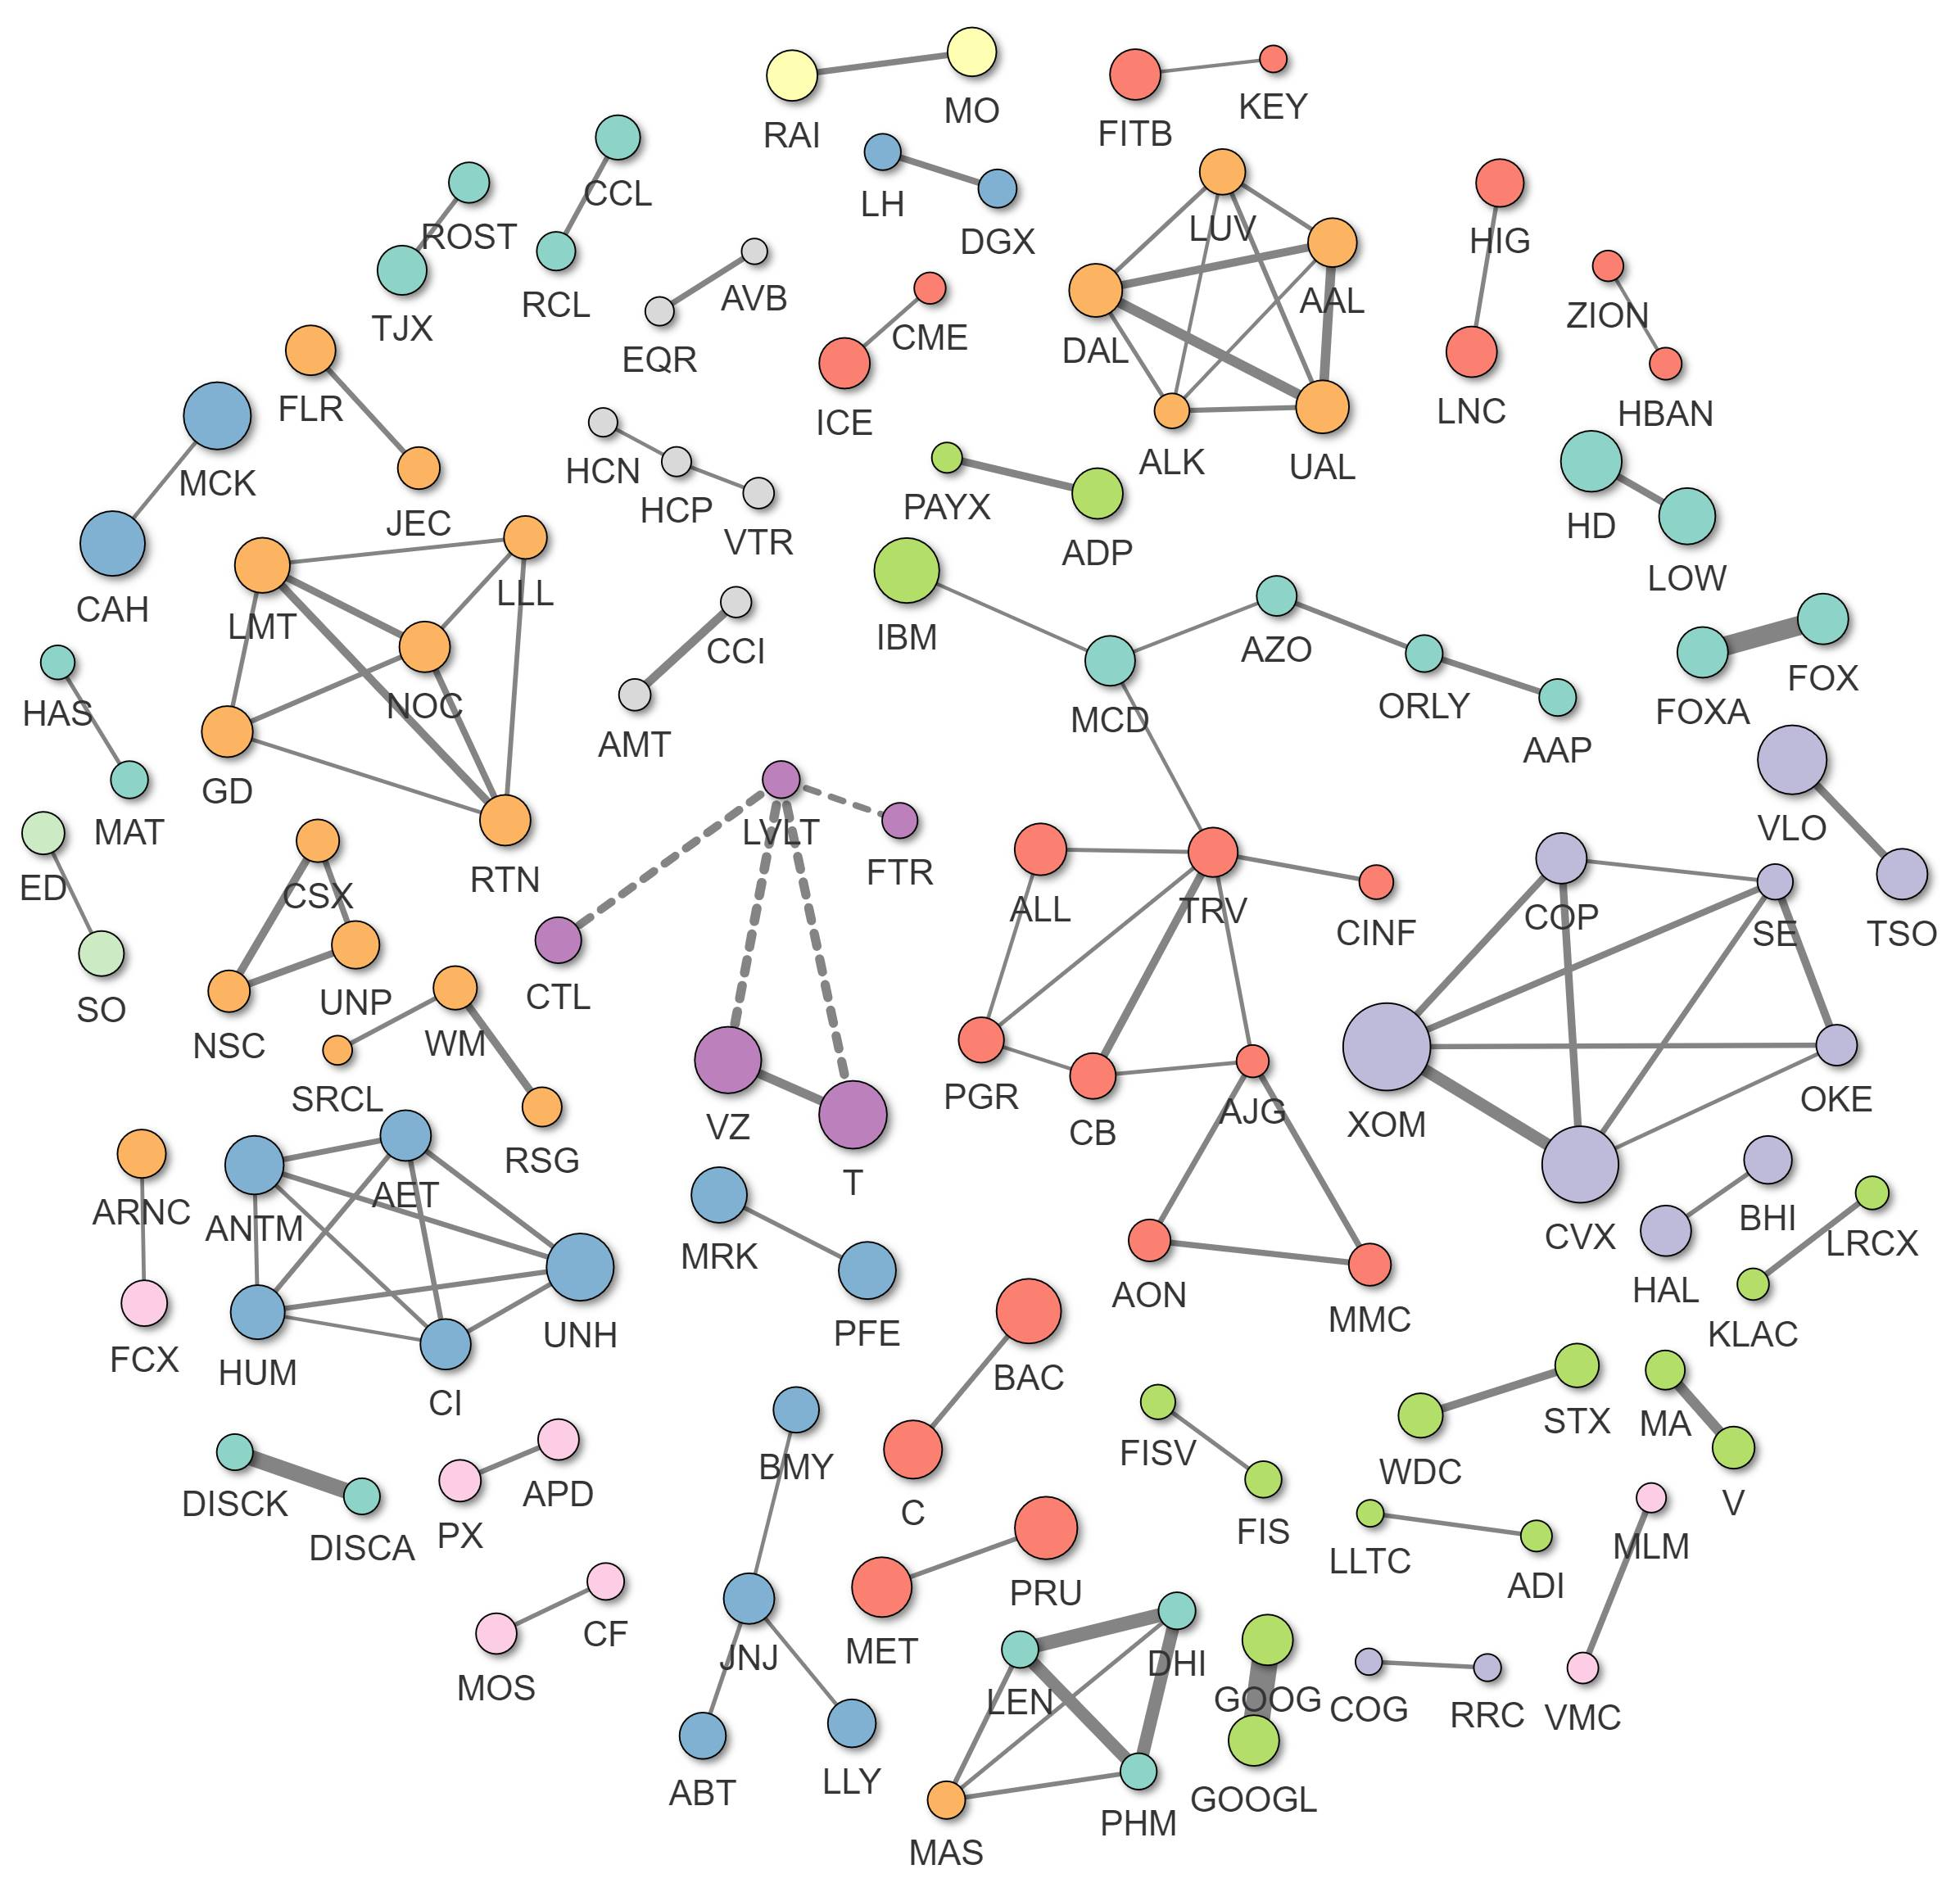
\includegraphics[width=\textwidth]{figures/regression/graph-corr-resid-999-42-with-neg.jpg}
    \end{subfigure}
    \vfill
    \begin{subfigure}{\textwidth}
        \centering
        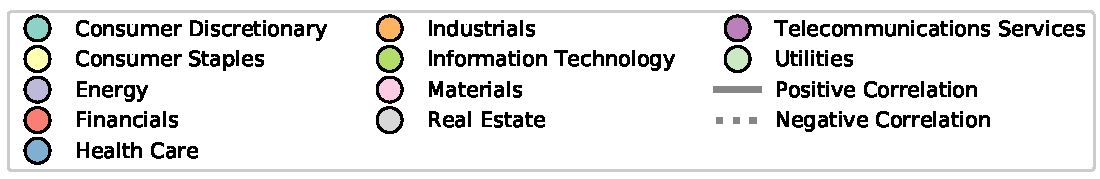
\includegraphics[width=\textwidth]{figures/graph-legend.pdf}
    \end{subfigure}

    \caption{Graph of the 109 greatest cross-correlations among stocks. Each node represents one stock which is labeled by the company's ticker symbol and coloured by the regarding industry section. Which color belongs to which industry is provided by the legend below. The node's size is determined by the total revenue for this company. Each edge between two nodes represents the cross-correlation $r$ between those stocks. More extreme values are indicated by a thicker edge and negative values by a dashed line.}
    \label{fig:graph-correlations}
\end{figure}

As indicated by the node colors, a large proportion of high correlations are observed among companies belonging to the same industry sectors. Only eight edges between two different sectors are present in this visualization. In terms of inter-industry connections, the node \emph{MCD} (\emph{McDonald's Corp.}) in the center of the graph is the strongest one since it is connected to nodes from three different industries. Investigation by financial news did not reveal an underlying relationship with the connected companies. Instead, this stock appears to be an appropriate strong representative component of the market performance and therefore is strongly linked to other important representative components like \emph{IBM} (\emph{International Business Machines}).

From the 109 edges selected for the graph, only four represent a negative correlation which all originate from the industry sector \emph{Telecommunications Services}. Further, it should be noted that there a three companies for which each one compromises two stocks. The reasoning for this is given in the previous Section~\ref{section:data}. Because two stocks of the same company are almost equal. these three correlation pairs reveal the highest $r$.

As denoted previously, this graph is not representative for the meaning of the measured cross-correlations. In order to examine this feature's usability, the final evaluation in Section~\ref{section:evaluation} will conduct a comparison with the extracted business relationships which are introduced in the following section.




% \begin{itemize}
%     \item Describe graph figure. Which correlation where chosen (99.9~\% Percentile: 0.3688, 123 nodes, 109 edges (incl 4 neg), 11 industries)
%     \item Collect insights: Only 8 edges between comps with different industry. Concluding, industry-correlation still exists
%     \item Not whole industries are connected but only pairs within industries giving evidence more meaningful relationships than just being in the same industry.
%     \item \emph{McDonald's Corp.} (node \emph{MCD} in the center of the graph) is the strongest connected node across several industries. Since investigation did not reveal an underlying relationship with the connected companies, this stocks instead appears to be an appropriate strong representative component of the market performance.
%     \item{Pairs of two stocks belonging to the same company are not removed}
% \end{itemize}




% \todo{Optional: Mutual Information, Cointegration, Granger Causality}

%%% Inspecting Cross-Dependencies
% Look into Dean2015 for more insights
% Calculate cross-correlation between residuals of stocks.
% Visually inspect change of cross-correlations over years? (like Mantegna)
% -> Inspect normalized MI and Pearson's r (as done by Dionisio)

% Cointegration & Causality Analysis
% Paper using Cointegration (Johansen Test): Kosapattarapim2017 https://drive.google.com/file/d/1wMcZlYGR69HT-JAH5382FIyfS4yh5gCC/view
% Paper using Granger Causality: Bollean2011 https://drive.google.com/file/d/1hv6CoM-_GnhDtVOGjhu-N3btCAIaA1an/view
% BDS (Bock, Dechert and Scheinkman[Hsieh 1989]) test (Dionisio2004) to test if variables are nonlinear independent
% Test for Unit Root, Cointegration, Granger Causality (bidir gc vs. simultaneity)



% Inspect correlation and prices in general for one specific quarter (e.g. 2011/02 appears to be bad for Energy)